\section{复数的三角表示}

本节要点:
\begin{itemize}
    \item 用三角表示理解复数的乘除。
\end{itemize}

~

三角表示及乘除运算如下:
\begin{align*}
&z=a+bi=r\left( \cos \theta +i\sin \theta \right) \\
&z_1\cdot z_2=r_1r_2\left[ \cos \left( \theta _1+\theta _2 \right) +i\sin \left( \theta _1+\theta _2 \right) \right] \\
&\frac{z_1}{z_2}=\frac{r_1}{r_2}\left[ \cos \left( \theta _1-\theta _2 \right) +i\sin \left( \theta _1-\theta _2 \right) \right]
\end{align*}
显然,复数的乘除的几何意义在于旋转。

~

\begin{example}[拓广探索9,难度:$\star $]
如下图,复平面内的$\bigtriangleup ABC$是等边三角形,它的两个顶点$A,B$的坐标分别为$\left( 1,0 \right) ,\left( 2,1 \right) $,求点$C$的坐标。
\end{example}

\begin{figure}[h]
\centering
\begin{minipage}{.49\textwidth}
\centering
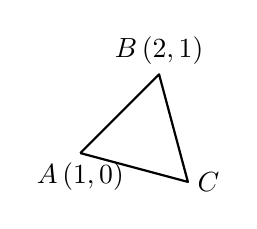
\begin{tikzpicture}[line join=round, scale=1]
\mydrawxy{-0.5}{3}{-0.5}{1.3}
\coordinate[label=below:{$A\left( 1,0 \right) $}] (A) at (1,0);
\coordinate[label=above:{$B\left( 2,1 \right) $}] (B) at (2,1);
\coordinate[label=right:{$C$}]                    (C) at (2.366,-0.366);
\draw[thick] (A)--(B)--(C)--(A);
\end{tikzpicture}
\end{minipage}
\begin{minipage}{.49\textwidth}
\centering
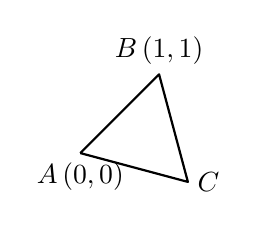
\begin{tikzpicture}[line join=round, scale=1]
\mydrawxy{-0.5}{2}{-0.5}{1.3}
\coordinate[label=below:{$A\left( 0,0 \right) $}] (A) at (0,0);
\coordinate[label=above:{$B\left( 1,1 \right) $}] (B) at (1,1);
\coordinate[label=right:{$C$}]                    (C) at (1.366,-0.366);
\draw[thick] (A)--(B)--(C)--(A);
\end{tikzpicture}
\end{minipage}
\end{figure}

解:

不妨平移坐标,如上右图,不难得到:
\begin{align*}
&z_B=\sqrt{2}\left( \cos \frac{\pi}{4}+i\sin \frac{\pi}{4} \right) \\
&z_C=\sqrt{2}\left[ \cos \left( -\frac{\pi}{12} \right) +i\sin \left( -\frac{\pi}{12} \right) \right]
\end{align*}
$C$在第四象限,于是:
\begin{align*}
&\cos \left( -\frac{\pi}{12} \right) =\sqrt{\frac{1+\cos \frac{\pi}{6}}{2}}=\sqrt{\frac{1}{2}+\frac{\sqrt{3}}{4}} \\
&\sin \left( -\frac{\pi}{12} \right) =-\sqrt{\frac{1-\cos \frac{\pi}{6}}{2}}=-\sqrt{\frac{1}{2}-\frac{\sqrt{3}}{4}} \\
&z_C=\sqrt{1+\frac{\sqrt{3}}{2}}-\sqrt{1-\frac{\sqrt{3}}{2}}i
\end{align*}
将坐标轴反向移回,得到$C$的最终坐标:
\[
z_C=\sqrt{1+\frac{\sqrt{3}}{2}}+1-\sqrt{1-\frac{\sqrt{3}}{2}}i
\]

\begin{tcolorbox}
本题也可以用向量求解,关键在于平移坐标系降低运算量。
\end{tcolorbox}

~

\begin{example}[拓广探索10,难度:$\star $]
如下图,已知平面内并列的三个全等的正方形,利用复数证明
\[
\angle 1+\angle 2+\angle 3=\frac{\pi}{2}
\]
\end{example}

\begin{figure}[h]
\centering
\begin{tikzpicture}[line join=round, scale=1.25]
\mydrawxy{-0.5}{3.5}{-0.5}{1.3}
\coordinate[label=below left:{$O$}] (A0) at (0,0);
\coordinate[label=below:     {$1$}] (A1) at (1,0);
\coordinate[label=below:     {$2$}] (A2) at (2,0);
\coordinate[label=below:     {$3$}] (A3) at (3,0);
\coordinate[label=left:      {$1$}] (B0) at (0,1);
\coordinate                         (B1) at (1,1);
\coordinate                         (B2) at (2,1);
\coordinate                         (B3) at (3,1);
\draw[thick] (A0)--(A3)--(B3)--(B0)--(A0) (A1)--(B1) (A2)--(B2) (A3)--(B3);
\draw[dashed] (A0)--(B1) (A0)--(B2) (A0)--(B3);
\pic["$1$",draw,angle radius=0.5cm,angle eccentricity=1.5] {angle=B0--B1--A0};
\pic["$2$",draw,angle radius=0.5cm,angle eccentricity=1.5] {angle=B0--B2--A0};
\pic["$3$",draw,angle radius=0.5cm,angle eccentricity=1.5] {angle=B0--B3--A0};
\end{tikzpicture}
\end{figure}

解:

令$z_1=1+i,z_2=2+i,z_3=3+i$,使用复数乘法的几何意义:
\[
z_1z_2z_3=\left( 1+i \right) \left( 2+i \right) \left( 3+i \right) =10i
\]
证毕。

\begin{tcolorbox}
本题考察复数乘法的几何意义,非常简单。
\end{tcolorbox}




